% =====================================================================
\chapter{Desarrollo Experimental}
\label{cap:desarrollo}

Este capítulo describe qué datos se usaron, cómo se limpiaron y unieron, qué mostró el
análisis exploratorio y cómo se especificó cada modelo. Los resultados de los modelos que
responden la pregunta de la tesina se presentan en el capítulo~\ref{cap:resultados}.

% ---------------------------------------------------------------------
\section{Materiales y métodos}
\label{sec:materiales}

\textbf{Fuentes de datos.} La tabla~\ref{tab:fuentes} resume las fuentes y sus ventanas. El
lado bursátil trabaja con dos ventanas: tres años para seleccionar las acciones y estudiar su
liquidez, y la ventana del corpus de noticias para la volatilidad y el régimen. La unión usa
el tramo en el que ambos lados tienen datos: aunque el corpus abarca desde enero de 2025, el
99,9\% de sus notas es posterior al 1 de mayo de 2025, de modo que la ventana común empieza en
la rueda del 5 de mayo de 2025.

\begin{table}[H]
\centering\small
\begin{tabularx}{\linewidth}{@{}L{3.2cm}YL{3.6cm}@{}}
\toprule
\textbf{Fuente} & \textbf{Qué aporta} & \textbf{Ventana} \\
\midrule
Yahoo Finance, \texttt{TICKER.BA} & Precio de apertura, máximo, mínimo, cierre y volumen de 53 candidatas (47 seleccionadas) & 03/05/2023 al 30/04/2026 (731 ruedas) \\
Yahoo Finance, \texttt{\^{}MERV} & Cierre del S\&P~Merval y calendario de ruedas de BYMA & 02/01/2025 al 30/04/2026 (323 ruedas) \\
Internet Archive (API CDX) & Capturas históricas de las secciones de economía de Ámbito, Clarín, Infobae, La Nación y TN & Enero de 2025 a mayo de 2026 \\
Mapas del sitio & Notas de Clarín, El Economista e iProfesional & Enero de 2025 a mayo de 2026 \\
Unión de ambos lados & Notas asignadas a ruedas, tono, atención y variables de mercado & 05/05/2025 al 30/04/2026 (244 ruedas) \\
\bottomrule
\end{tabularx}
\caption{Fuentes de datos y ventanas temporales. Fuente: elaboración propia.}
\label{tab:fuentes}
\end{table}

\textbf{Entorno.} Python 3 con \texttt{pandas}, \texttt{numpy}, \texttt{scipy},
\texttt{statsmodels} 0.14.6 y \texttt{matplotlib} para el lado bursátil y la unión;
\texttt{yfinance} para la descarga de precios. El lado de noticias tiene su propio entorno
(Python 3.13) con \texttt{requests}, \texttt{beautifulsoup4}, \texttt{trafilatura},
\texttt{spacy} 3.8 con el modelo \texttt{es\_core\_news\_lg}, \texttt{transformers} y
\texttt{torch} con aceleración por GPU. El etiquetado de oraciones y la verificación de
duplicados semánticos se hicieron con modelos de lenguaje abiertos (Gemma y Qwen3) servidos
localmente con Ollama.

\textbf{Organización y reproducibilidad.} Cada paso es una carpeta con un único script, sus
resultados en CSV, un archivo de controles automáticos (\texttt{verificaciones.csv}) y su
documentación en PDF. Ningún paso modifica los archivos de otro: cada uno lee lo que necesita y
escribe en su propia carpeta. La unión completa se rehace con un solo comando
(\texttt{python correr\_todo.py}, en \carpeta{Unión/09_entrega_final}), que corre los pasos
en orden, verifica los controles y compara la huella de cada archivo de resultados con la
corrida anterior: los 64 archivos salen idénticos y los 66 controles pasan. El anexo~\ref{anx:repro}
detalla la estructura de carpetas.

\textbf{Datos de terceros.} Las notas periodísticas pertenecen a sus medios y se usaron
únicamente con fines académicos: el análisis trabaja con medidas agregadas (tono, cantidad,
menciones) y no reproduce las notas. Los precios provienen de Yahoo Finance, también con fines
académicos. El acceso autenticado a la API de Internet Archive usa credenciales guardadas en un
archivo de configuración externo, fuera del código.

% ---------------------------------------------------------------------
\subsection{Recolección de los datos}
\label{sec:recoleccion}

\subsubsection{Corpus de noticias}

El corpus se recolectó de las secciones de economía y finanzas de siete portales, con dos
métodos según la disponibilidad de cada fuente (sección~\ref{sec:tec-adquisicion}): la
Wayback Machine para Ámbito Financiero (Economía y Finanzas), Clarín (Economía), Infobae, La
Nación y TN, y los mapas del sitio para Clarín, El Economista e iProfesional. Clarín se cubrió
con ambos métodos: la ventana más profunda por Wayback Machine y las notas más recientes por
el mapa del sitio. Cada nota se guardó con su sitio, fecha y hora de publicación, título,
bajada, contenido y etiquetas. El corpus final tiene 14.012 artículos, unos 63 millones de
caracteres (alrededor de 4.500 por artículo), publicados entre enero de 2025 y mayo de 2026
(tabla~\ref{tab:corpus}). En la práctica empieza en mayo de 2025: 14.001 de los 14.012 son
del 1 de mayo de 2025 en adelante, probablemente porque tanto la retención de los mapas del
sitio como las capturas de la Wayback Machine se concentran en los meses más recientes.

\subsubsection{Panel de acciones}

Se partió de 53 candidatas del Panel General y del Panel Líderes de BYMA: las 20 del
S\&P~Merval más 33 de sectores similares. Para cada una se descargó la serie diaria de tres
años y se midieron dos cosas: cuántas ruedas tiene y qué porcentaje de ellas tuvo volumen
mayor que cero. El criterio de selección exige las dos condiciones a la vez:

\begin{itemize}
  \item \textbf{Cobertura completa del calendario:} las 731 ruedas de la ventana, sin
        excepciones.
  \item \textbf{Al menos 90\% de días con volumen real.} Un día con volumen cero no es un dato
        faltante: Yahoo entrega la fila, con el precio pegado al último que operó. Por eso el
        criterio no puede mirar solo el calendario.
\end{itemize}

Pasaron 47 de las 53, incluidas las 20 del S\&P~Merval. Las seis que quedaron afuera son
Carboclor (462 ruedas y 39\% de días con volumen), Holcim Argentina (67,2\%), Polledo
(50,2\%), Instituto Rosenbusch (87,3\%) y dos tickers sin datos en Yahoo: NII Holdings y TGLT,
que es la misma empresa que hoy cotiza como GCDI, incluida en el panel. Los nombres y sectores
se verificaron contra la ficha de cada ticker; los \textit{holdings} diversificados (Cresud,
Sociedad Comercial del Plata, Garovaglio y Zorraquín) se clasificaron como Conglomerado.

% ---------------------------------------------------------------------
\subsection{Limpieza y preparación de los datos}
\label{sec:limpieza}

\subsubsection{Depuración del corpus}

La auditoría del corpus encontró cinco problemas, cada uno con su solución
(tabla~\ref{tab:depuracion}).

\begin{table}[H]
\centering\small
\begin{tabularx}{\linewidth}{@{}L{3.4cm}YY@{}}
\toprule
\textbf{Problema} & \textbf{Qué se encontró} & \textbf{Solución} \\
\midrule
Duplicados exactos & 205 notas de Clarín descargadas dos veces, por Wayback Machine y por el mapa del sitio & Una copia por URL (la del sitio); los recolectores verifican la URL contra todo el corpus \\
Publicación cruzada & 208 grupos de título repetido; 175 se descartaron por estar a más de 48 horas (columnas recurrentes) & Los 33 grupos restantes (68 notas) se verificaron con Qwen3: 14 republicaciones reales \\
Metadatos faltantes & Sin autor ni palabras clave en iProfesional y sin fecha en 194 notas de El Economista, por un error de parseo del JSON-LD & Parseo tolerante; 192 notas reales se volvieron a descargar y recuperaron su fecha \\
Contenido que no es noticia & 2 páginas índice, 9 páginas de suscripción y 6 notas fuera de la ventana (fechadas por su última modificación) & Se eliminaron; los recolectores filtran por fecha de publicación efectiva \\
Plantillas & 65 grupos (479 notas) con el mismo comienzo; cuatro plantillas de El Economista concentran 325 notas con sentimiento constante & Se eliminaron 419 notas (2,9\%): el corpus pasó de 14.431 a 14.012 \\
\bottomrule
\end{tabularx}
\caption{Problemas del corpus y cómo se resolvieron. Fuente: elaboración propia a partir de
la auditoría del lado de noticias (\carpeta{Lado Noticias/noticias}).}
\label{tab:depuracion}
\end{table}

Las plantillas merecen un comentario. Notas como el reporte diario «Dólar hoy» tienen fecha y
cotizaciones propias, pero el modelo de sentimiento les asignaba siempre el mismo valor, con
desvío cero entre decenas de notas: el valor dependía de la parte fija del texto y no de la
información del día. Replicado durante meses, ese valor sesgaba el promedio diario. En los
grupos de menos de 11 notas se conservó la más antigua (83 eliminadas); en los de 11 o más,
cuyo cuerpo es relleno, se eliminaron todas (336). Una sola nota de 2014 mal fechada, además,
estiraba la serie diaria a 4.186 días; tras la depuración la serie abarca 487 días.

\subsubsection{Depuración de los precios}

\begin{itemize}
  \item \textbf{Calendario real de BYMA.} Yahoo agrega a cada acción una fila en los feriados
        (precio pegado, volumen cero) que el índice no tiene. Se descargó primero el
        \texttt{\^{}MERV} y se usó su lista de fechas como calendario para todas las acciones.
  \item \textbf{Fallas intermitentes.} Algunos tickers daban «sin datos» en una corrida y
        datos completos en la siguiente; el script reintenta hasta tres veces antes de
        descartarlos.
  \item \textbf{Eventos corporativos mal ajustados.} Buscando retornos diarios mayores a
        $\pm50\%$ aparecieron dos errores de Yahoo: el 16/12/2024 de SEMI quedó sin dividir
        por el \textit{split} de 4,227 (se corrigió ese día), y el dividendo en acciones de
        AGRO de noviembre de 2023 no se aplicó a los precios anteriores, lo que mostraba una
        caída falsa de 88\% (los precios hasta el 02/11/2023 se dividieron por 2,1). Los
        saltos grandes de GCDI, CELU y RIGO se verificaron como reales: el precio se sostiene
        o viene con volumen muy por encima de lo normal.
\end{itemize}

\subsubsection{Cada nota a su rueda}
\label{sec:alineacion}

Las noticias se publican a cualquier hora, pero el precio se forma solo en las ruedas, de lunes
a viernes de 11:00 a 17:00. Para medir si una nota mueve el precio hay que compararla con el
primer precio que pudo verse afectado por ella. Una nota del martes a las 20:00 sale con el
mercado cerrado: la primera vez que alguien puede operar con esa información es el miércoles.
Se aplicó la siguiente regla:

\begin{itemize}
  \item Todas las horas se pasaron a hora argentina: Clarín, Infobae y La Nación informan la
        hora en UTC, y 95 notas nocturnas cambian de fecha con la conversión.
  \item Una nota publicada antes de las 17:00 de un día con rueda cuenta para esa rueda.
  \item Una nota publicada a las 17:00 o después cuenta para la rueda siguiente.
  \item Una nota publicada en un día sin rueda (fin de semana o feriado) cuenta para la
        primera rueda posterior.
\end{itemize}

El 59,8\% de las notas quedó en su mismo día, el 24,8\% pasó a la rueda siguiente por salir
después del cierre y el 15,4\% por salir en un día sin rueda (tabla~\ref{tab:alineacion}).
Dentro de la ventana quedaron 13.925 notas; las 10 de enero a marzo de 2025 y las 77 del
cierre del 30/04/2026 en adelante quedan afuera. Las 244 ruedas reciben noticias: mínimo 12,
mediana 55 y máximo 145 (figura~\ref{fig:u1}).

\begin{table}[H]
\centering\small
\begin{tabular}{@{}lrr@{}}
\toprule
\textbf{Dónde quedó cada nota} & \textbf{Notas} & \textbf{\%} \\
\midrule
En su mismo día (antes de las 17:00 de un día con rueda) & 8.332 & 59,8 \\
En la rueda siguiente, por salir después del cierre & 3.451 & 24,8 \\
En la rueda siguiente, por salir en un día sin rueda & 2.142 & 15,4 \\
\midrule
Total dentro de la ventana & 13.925 & 100,0 \\
\bottomrule
\end{tabular}
\caption{Asignación de las notas a las ruedas con la regla de las 17:00. Fuente: elaboración
propia (\carpeta{Unión/01_alineacion_noticias_ruedas}).}
\label{tab:alineacion}
\end{table}

\begin{figure}[H]
\centering
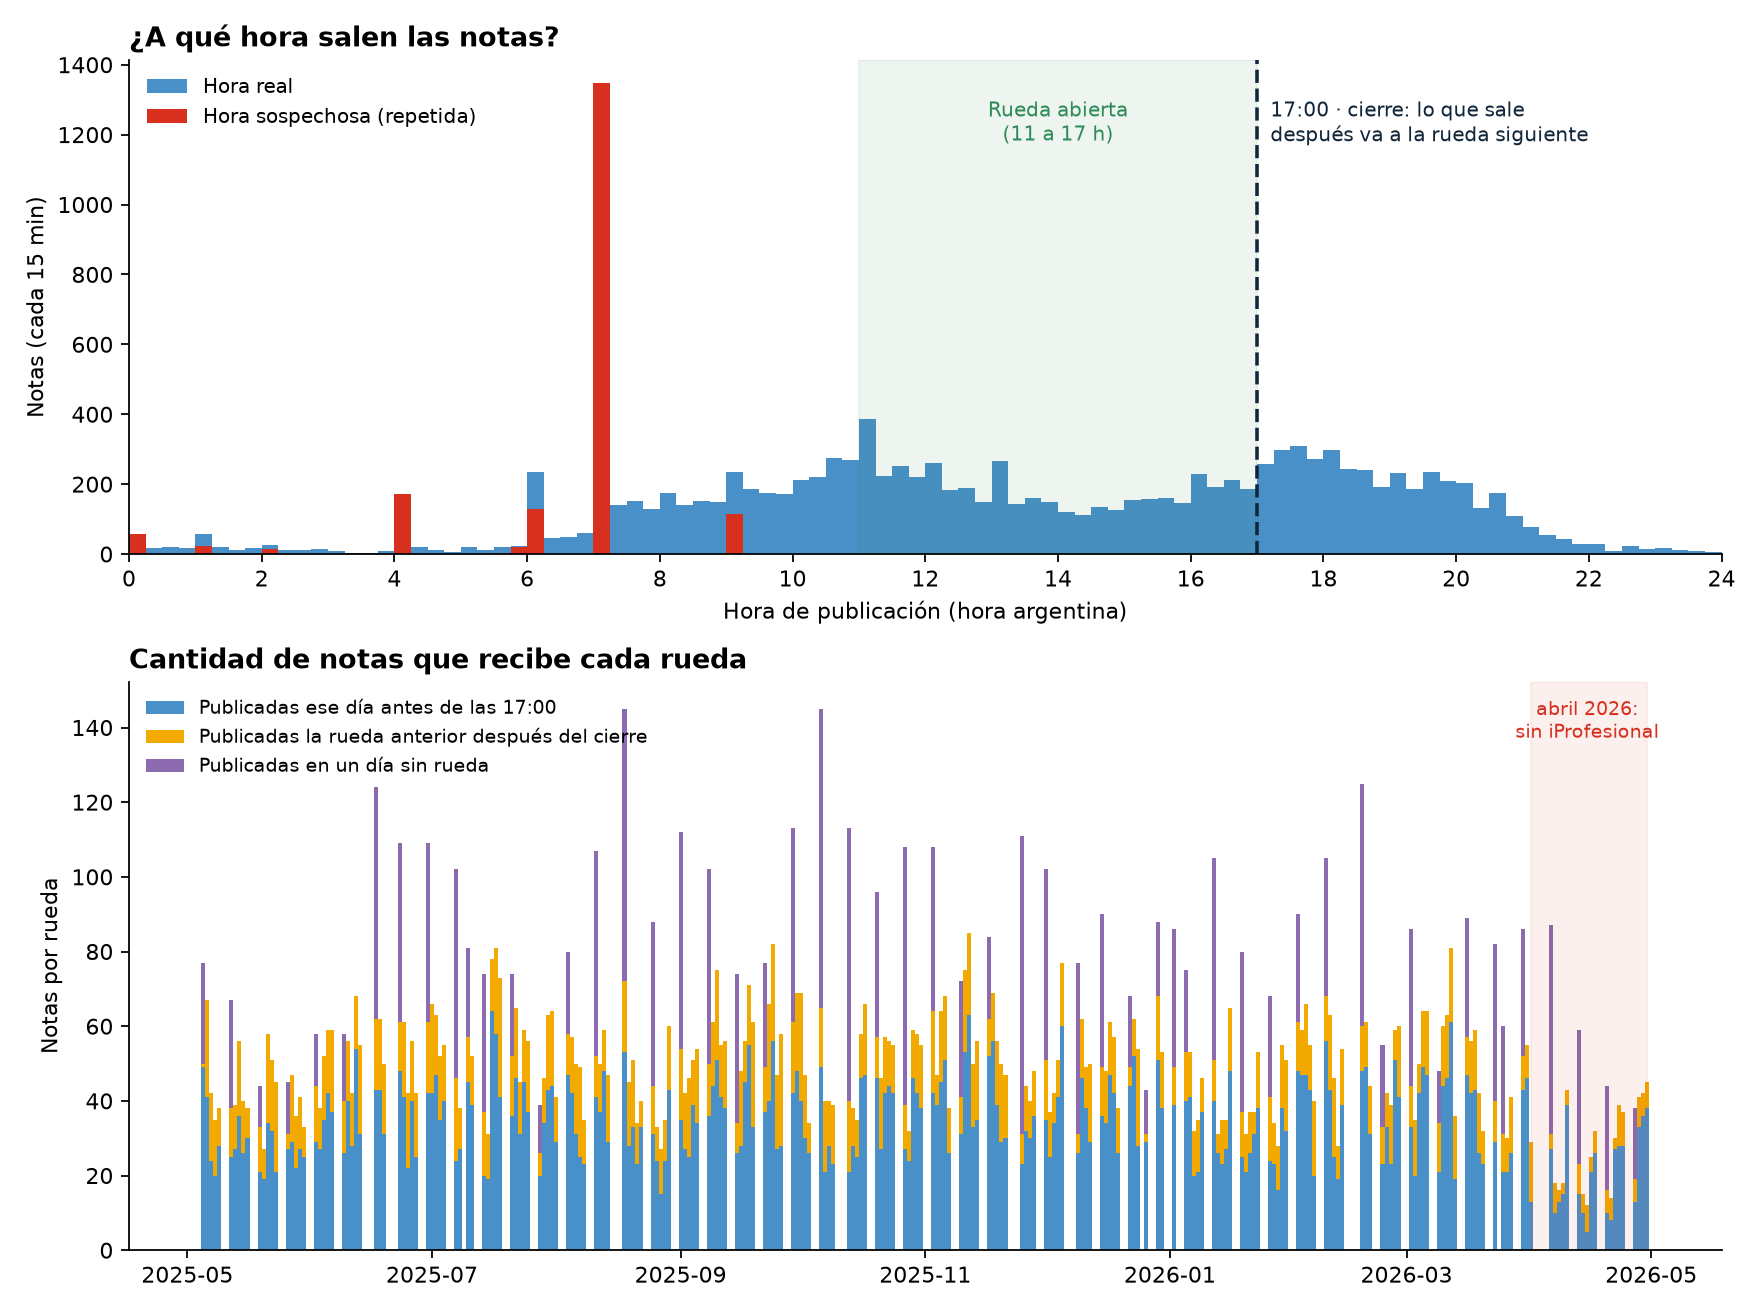
\includegraphics[width=0.88\linewidth]{u1_alineacion.png}
\caption{Arriba: hora de publicación de las notas, con la rueda sombreada y el cierre de las
17:00; en rojo, horas repetidas que no pueden ser reales. Abajo: notas que recibe cada rueda,
según de dónde vienen. Fuente: elaboración propia (\carpeta{Unión/01_alineacion_noticias_ruedas}).}
\label{fig:u1}
\end{figure}

\textbf{Horas sospechosas.} El 13,4\% de las notas (1.881) tiene una hora que se repite
demasiado dentro de su portal —más del 3\% de sus notas a un mismo minuto—, como las 07:00 de
Clarín o las 00:00 de Ámbito. No es la hora real sino una hora por defecto del sitio. Esas
notas se marcaron y, en la prueba de robustez, los resultados se repitieron sin ellas
(sección~\ref{sec:res-u8}). El anexo~\ref{anx:alineacion} lista las horas detectadas.

\subsubsection{Tono, atención y ruedas de tono extremo}
\label{sec:tono-rueda}

Con cada nota asignada a su rueda se armaron tres series por rueda:

\begin{itemize}
  \item \textbf{Tono:} el promedio del sentimiento neto de las notas de la rueda, con igual
        peso por nota. El sentimiento neto de una nota es el porcentaje de sus oraciones
        positivas menos el de negativas (sección~\ref{sec:finbeto-modelo}). Como cada portal
        tiene su propio tono promedio, se armó también una versión \textit{ajustada por
        portal}, restando a cada nota el promedio de su portal; las dos versiones tienen
        correlación 0,995.
  \item \textbf{Atención:} la cantidad de notas de la rueda comparada con lo habitual. Una
        rueda que viene de un fin de semana junta más notas (mediana de 50 notas en ruedas que
        cubren un día, 83 en las que cubren tres y 111 en las que cubren cuatro). Por eso la
        cantidad se compara primero con la mediana de las ruedas que cubren los mismos días y
        después con el nivel de las 20 ruedas previas. En la \textit{atención anormal}
        resultante, 0 es lo habitual, $+0{,}69$ el doble de notas y $-0{,}69$ la mitad.
  \item \textbf{Ruedas de tono extremo:} las ruedas cuyo tono se aparta mucho de lo habitual.
\end{itemize}

Para elegir la regla de las ruedas de tono extremo se compararon dos familias
(tabla~\ref{tab:reglas}). La primera mide lo habitual con el desvío de los días previos,
como la serie diaria del lado de noticias; la segunda, \textit{por muestreo}, pregunta cuánto
podría moverse el promedio del día solo por azar, según cuántas notas tiene: con 100 notas, una
diferencia de 9 puntos es creíble; con 16, puede ser casualidad, como el margen de error de una
encuesta. Para saber si una regla detecta algo se mezclaron las notas al azar entre las ruedas,
conservando cuántas tiene cada una, y se contó cuántos shocks marcaba cada regla. El criterio,
fijado antes de mirar el resultado, fue usar 20 ruedas de referencia y el umbral que más shocks
detecta con a lo sumo 20\% de falsos esperados.

\begin{table}[H]
\centering\footnotesize
\begin{tabular}{@{}lccc@{}}
\toprule
\textbf{Regla} & \textbf{Umbral} & \textbf{Noticias reales} & \textbf{Notas mezcladas al azar} \\
\midrule
Desvío de los días previos & 1,5 & 50 & 35,4 \\
Desvío de los días previos & 2,0 & 15 & 16,1 \\
Desvío de los días previos & 2,5 & 4 & 7,1 \\
Por muestreo & 2,0 & 35 & 11,6 \\
\textbf{Por muestreo (elegida)} & \textbf{2,5} & \textbf{19} & \textbf{3,5} \\
Por muestreo & 3,0 & 8 & 0,8 \\
Regla de la serie diaria (7 días, incluye el día) & 1,5 & 33 & 25,8 \\
\bottomrule
\end{tabular}
\caption{Shocks de tono que marca cada regla con las noticias reales y con las notas
mezcladas al azar (promedio de 300 mezclas). Fuente: elaboración propia
(\carpeta{Unión/02_sentimiento_por_rueda}).}
\label{tab:reglas}
\end{table}

La regla por desvío de los días previos marca casi lo mismo que el azar. La regla por muestreo
con umbral 2,5 marca 19 ruedas de tono extremo (10 positivas y 9 negativas), contra 3,5
esperables por azar. Hay un matiz: las notas de un mismo día no son independientes, porque
todos los medios hablan de los mismos temas, y por eso los días varían más de lo que predice
su cantidad de notas. Teniéndolo en cuenta, se esperarían unas 19 ruedas así. Por eso las 19
se interpretan como \textit{las ruedas de tono más extremo del período} (el 8\% más alejado de
lo habitual) y no como días estadísticamente excepcionales. El análisis principal (VAR y
Granger) no depende de esta regla: usa la serie completa de tono.

La regla de la serie diaria original incluye al propio día en la ventana de siete días con
que se calcula lo habitual. Eso acota el desvío máximo alcanzable a
$(7-1)/\sqrt{7} \approx 2{,}27$ \citep{shiffler1988}, y es uno de los motivos por los que la
unión redefinió la banda sin el día evaluado.

\begin{figure}[H]
\centering
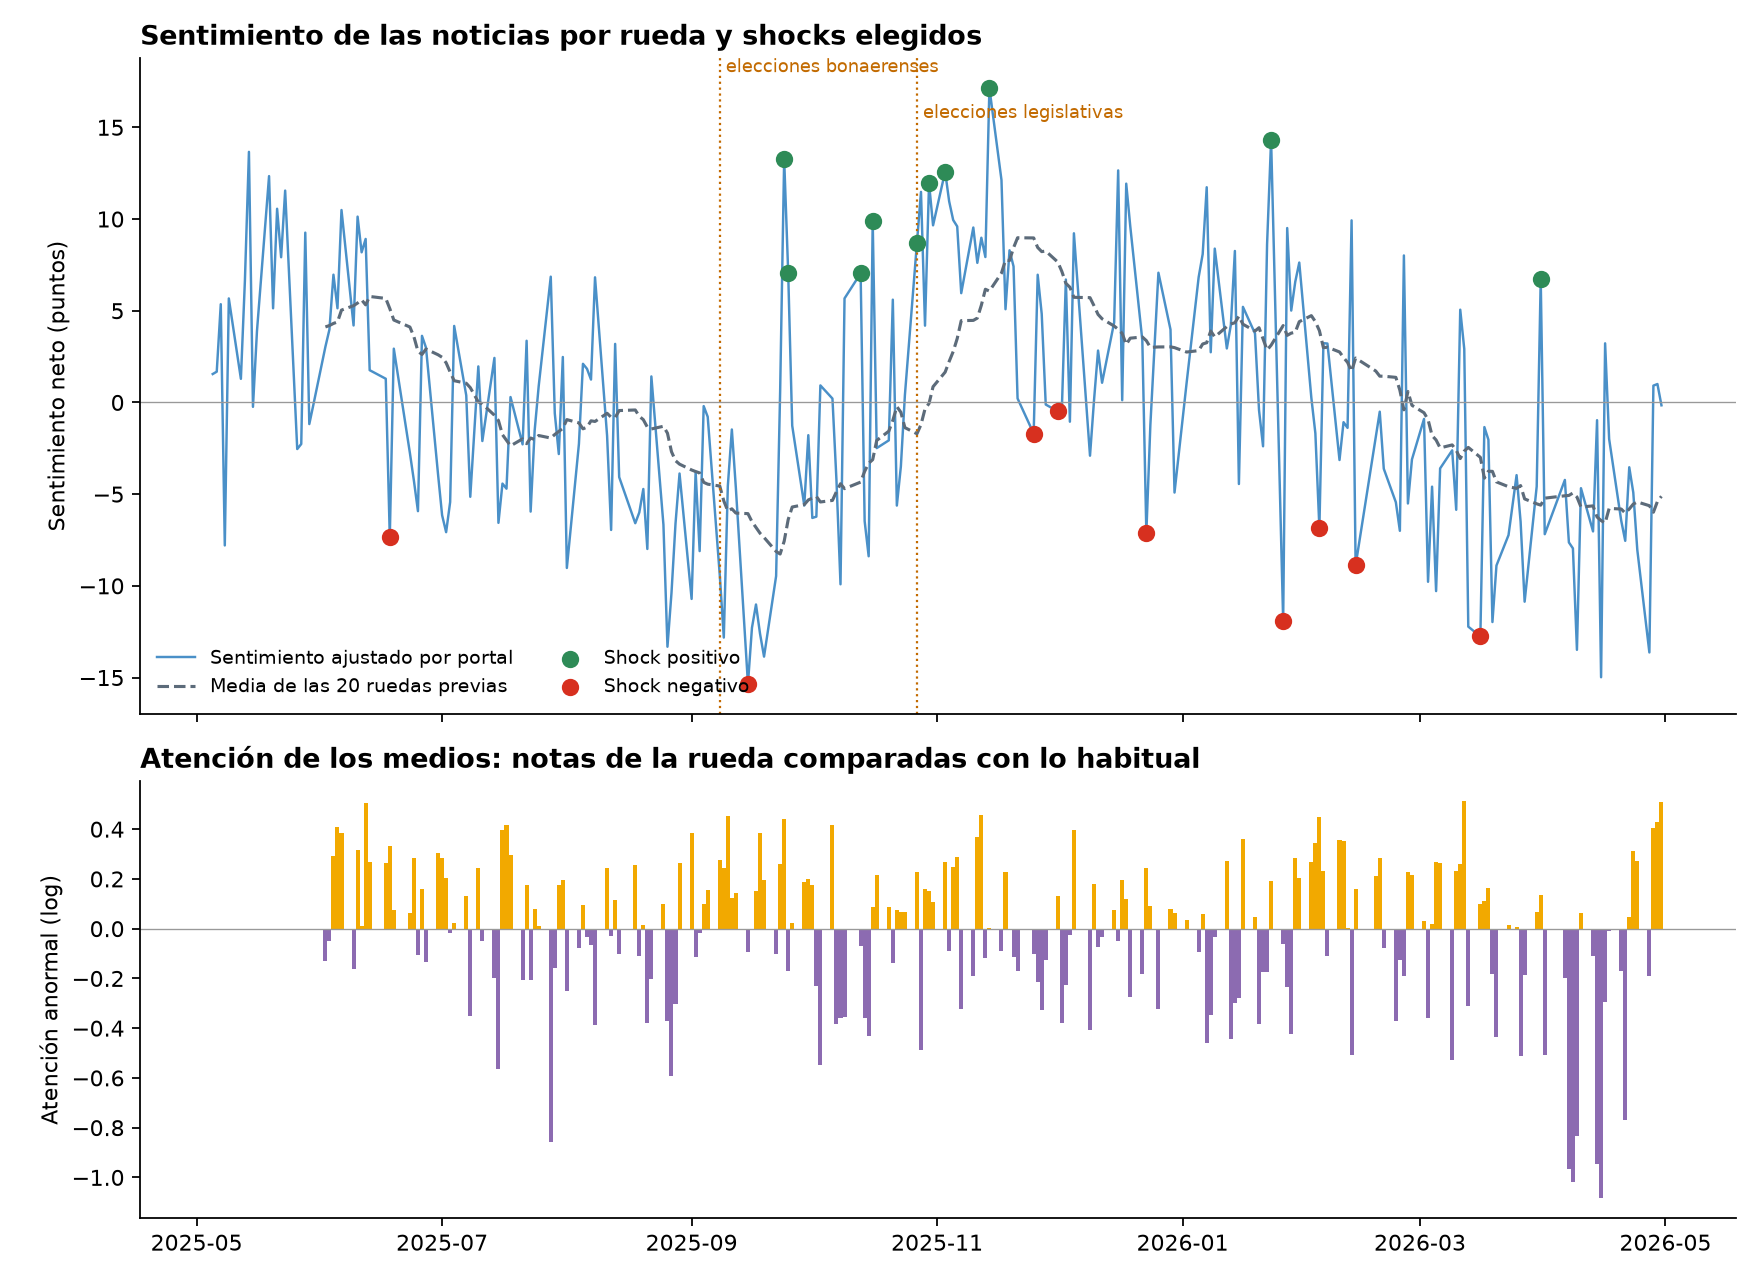
\includegraphics[width=0.88\linewidth]{u2_serie.png}
\caption{Arriba: tono de cada rueda (ajustado por portal), su media de las 20 ruedas previas y
las ruedas de tono extremo. Abajo: atención anormal de los medios. Fuente: elaboración propia
(\carpeta{Unión/02_sentimiento_por_rueda}).}
\label{fig:u2}
\end{figure}

\subsubsection{Tono de cada empresa}

El tono de una empresa en una rueda se calculó con el cruce entre las menciones del NER y el
sentimiento de cada oración (sección~\ref{sec:ner-modelo}): (oraciones positivas $-$
oraciones negativas) / oraciones que mencionan a la empresa $\times$ 100. Cada oración cuenta
para la rueda de su nota, y una oración que menciona dos veces a la misma empresa cuenta una
sola vez. Se unieron 240.811 de 242.312 oraciones con entidades (99,38\%). Si una empresa no
aparece en una rueda, su tono queda vacío y la marca \var{hubo\_noticia} vale 0: completar
con 0 la haría parecer neutra. Agrupando por fecha en lugar de por rueda, el cálculo reproduce
fila por fila la serie diaria por empresa del lado de noticias.

Un aviso para los modelos: en las 17 empresas con tono propio, una rueda con noticias tiene
una mediana de dos oraciones que la mencionan, y en el 37\% de esas ruedas hay una sola. Ese
día el tono sale todo o nada ($+100$, $-100$ o 0). Por eso el modelo usa el \textit{tono
propio} encogido hacia el mercado (ecuación de la sección~\ref{sec:tec-modelos}), que vale 0
cuando no hay noticias y confía más en las ruedas con más oraciones.

\begin{figure}[H]
\centering
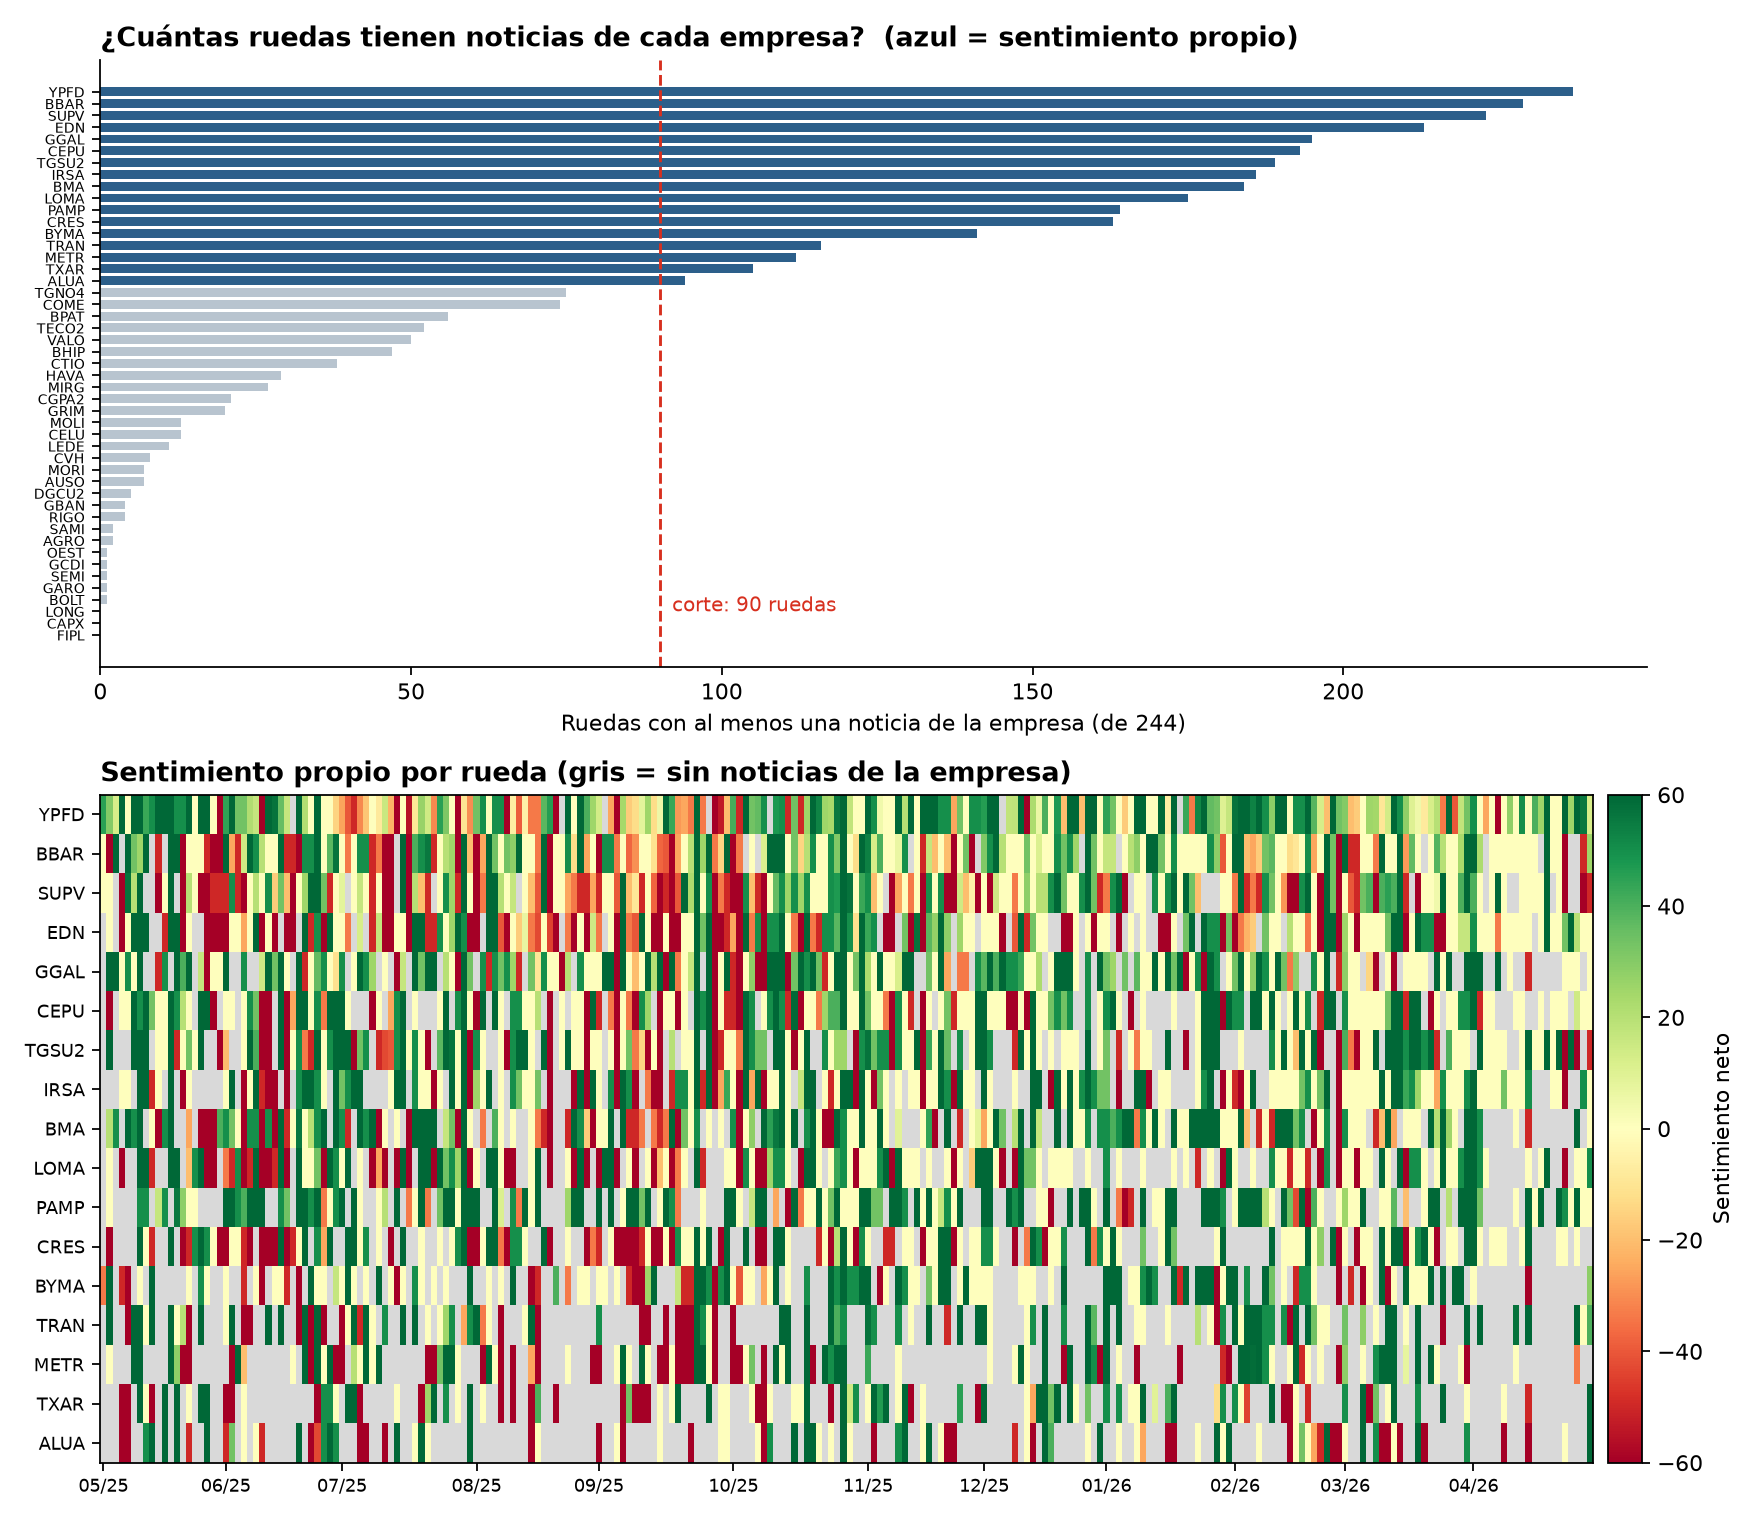
\includegraphics[width=0.85\linewidth]{u3_cobertura.png}
\caption{Arriba: ruedas con al menos una noticia de cada empresa (en azul, las 17 con tono
propio). Abajo: tono propio de esas 17 empresas en cada rueda. Fuente: elaboración propia
(\carpeta{Unión/03_sentimiento_por_empresa}).}
\label{fig:u3}
\end{figure}

\subsubsection{Datasets unificados}

Todo lo que usan los modelos quedó en dos tablas, para que ningún modelo arme su propio cruce:
\var{dataset\_mercado.csv}, con una fila por rueda (244 filas), y \var{dataset\_panel.csv},
con una fila por acción y rueda (11.468 filas). El diccionario de variables está en el
anexo~\ref{anx:diccionario}. Tres decisiones definen sus variables:

\begin{itemize}
  \item \textbf{Volumen anormal.} El volumen en bruto no sirve para comparar: cada acción tiene
        su propio nivel y los montos en pesos crecen con la inflación. Se usa
        $\log(1+\text{volumen}_t)$ menos el promedio de esa cantidad en las 20 ruedas previas
        de la misma acción; para el mercado, lo mismo con el monto operado total de las 47.
  \item \textbf{Tono anormal.} El tono de la rueda menos el promedio de las 20 ruedas previas.
        Es la variable de tono del VAR (sección~\ref{sec:multivariado}).
  \item \textbf{Marcas de días especiales.} Se marcaron las dos ruedas electorales (08/09 y
        27/10/2025), las 40 ruedas de su eco en el VIX y el régimen, y las 20 ruedas de abril
        de 2026, cuando el corpus casi no tiene notas de iProfesional por un hueco de
        recolección. Las marcas no cambian ningún dato: sirven para analizar esos días aparte.
\end{itemize}

% ---------------------------------------------------------------------
\subsection{Análisis univariado}
\label{sec:univariado}

\textbf{Retorno del mercado.} En las 244 ruedas de la unión, el retorno diario del
S\&P~Merval promedió 0,16\%, con un desvío de 2,79\%. Los extremos son los dos días
electorales: $-13{,}25\%$ el 08/09/2025 y $+21{,}77\%$ el 27/10/2025. El VIX argentino
promedió 41,9\% en esa ventana (tabla~\ref{tab:descriptivos}).

\textbf{Volatilidad por acción.} La volatilidad promedio de las 47 acciones fue de 55,1\%,
contra 44,0\% del VIX en los mismos 323 días: cada acción sola es más nerviosa que el índice,
que diversifica. La más calma fue Mirgor (36,2\%) y la más volátil, Celulosa Argentina
(104,6\%) (figura~\ref{fig:ranking}). Por sector, Real Estate fue el más calmo (42,5\%) y
Utilities el más volátil (60,5\%).

\begin{figure}[H]
\centering
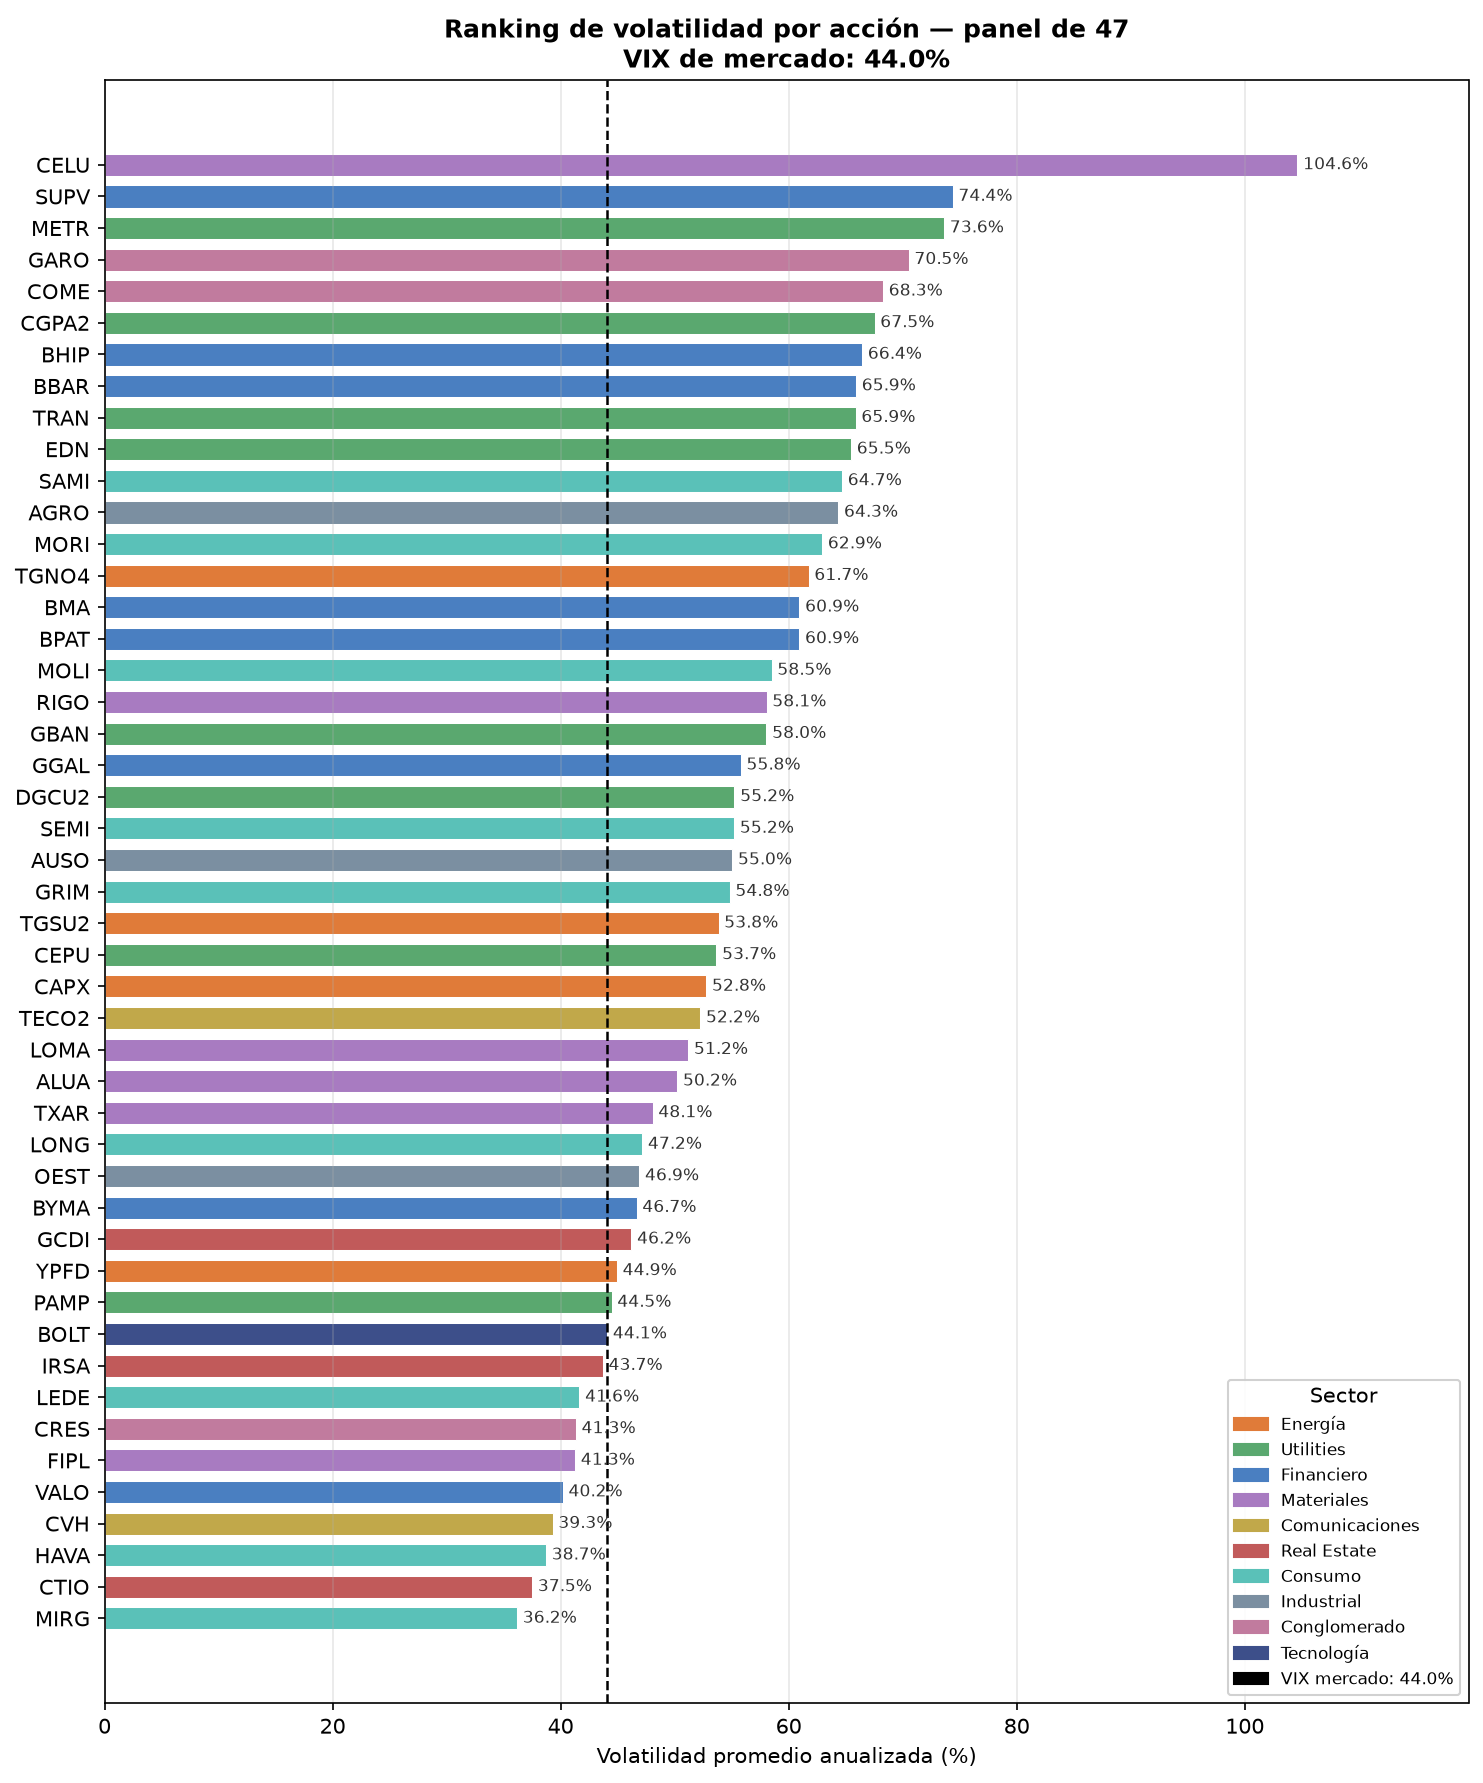
\includegraphics[width=0.66\linewidth]{ranking_volatilidad.png}
\caption{Volatilidad promedio de las 47 acciones, coloreada por sector, con el VIX argentino
como referencia (2/1/2025 al 30/4/2026). Fuente: elaboración propia
(\carpeta{Lado Bursatil/05_volatilidad_ranking}).}
\label{fig:ranking}
\end{figure}

Se marcaron como \textit{picos propios} los tramos de tres días o más en que la volatilidad
de una acción supera al VIX por más de 60 puntos mientras el VIX está por debajo de 50\%: la
acción muy alterada en un mercado tranquilo. De 19 tramos, 12 empiezan justo cuando el VIX cae
de golpe por el eco de 20 ruedas, y no se cuentan. Quedan 7 tramos genuinos en cuatro acciones
(CELU, SAMI, GARO y RIGO), candidatos a eventos propios de cada empresa.

\textbf{Tono de las noticias.} El tono medio de las 244 ruedas fue de 3,9 puntos, con un
desvío de 7,0: las noticias económicas son, en promedio, levemente positivas. La rueda más
negativa fue la del 15/04/2026 ($-13{,}5$) y la más positiva, la del 14/11/2025 ($+22{,}1$).
El tono de una rueda se parece al de la anterior (autocorrelación 0,47): el clima de las
noticias cambia de a poco. A nivel de oración, de las 399.803 oraciones clasificadas, el 36,7\%
es neutra, el 27,1\% positiva, el 24,1\% negativa y el 12,1\% mixta.

\textbf{Cantidad de notas.} Las ruedas reciben entre 12 y 145 notas, con mediana de 55. Los
lunes reciben el fin de semana: mediana de 85 notas, contra 50 el resto de los días. La rueda
con más notas es la del 18/08/2025 (145), que junta cuatro días porque el viernes anterior fue
feriado. Abril de 2026 recibe menos notas por el hueco de recolección de iProfesional.

\textbf{Menciones de empresas.} YPF es la empresa más mencionada: aparece en 237 de las 244
ruedas. Le siguen BBVA (229), Supervielle (223), Edenor (213) y Galicia (195). Tres empresas
del panel no tienen ninguna mención (CAPX, FIPL y LONG) y otras 16 tienen menos de 10 ruedas
con noticias. El tono acumulado de las oraciones que mencionan a cada empresa va de $-0{,}5$
(Aluar) a $+40{,}8$ (Pampa Energía).

\begin{table}[H]
\centering\small
\begin{tabular}{@{}lrrrrr@{}}
\toprule
\textbf{Variable} & \textbf{Filas} & \textbf{Media} & \textbf{Desvío} & \textbf{Mínimo} & \textbf{Máximo} \\
\midrule
Retorno del S\&P~Merval (\%) & 244 & 0,16 & 2,79 & $-$13,25 & 21,77 \\
VIX argentino (\%) & 244 & 41,87 & 17,04 & 15,40 & 90,99 \\
Monto operado anormal (log) & 244 & 0,00 & 0,46 & $-$2,21 & 1,44 \\
Tono de las noticias & 244 & 3,91 & 7,00 & $-$13,54 & 22,10 \\
Tono ajustado por portal & 244 & $-$0,07 & 6,87 & $-$15,34 & 17,15 \\
Tono anormal & 224 & $-$0,51 & 6,01 & $-$16,94 & 20,97 \\
Notas por rueda & 244 & 57,07 & 22,87 & 12,00 & 145,00 \\
Atención anormal (log) & 224 & $-$0,01 & 0,30 & $-$1,08 & 0,51 \\
Retorno de cada acción (\%) & 11.468 & 0,12 & 3,86 & $-$39,57 & 53,96 \\
Volumen anormal de cada acción (log) & 11.468 & $-$0,02 & 0,77 & $-$12,68 & 4,79 \\
Tono de la empresa (si hubo noticia) & 3.489 & 12,57 & 62,39 & $-$100,00 & 100,00 \\
Oraciones que mencionan a la empresa & 11.468 & 0,96 & 3,13 & 0,00 & 185,00 \\
Tono propio (17 empresas) & 4.148 & 1,67 & 9,17 & $-$40,67 & 49,05 \\
\bottomrule
\end{tabular}
\caption{Estadísticos descriptivos de las variables principales en la ventana de la unión
(05/05/2025 al 30/04/2026). El tono anormal y la atención tienen 224 filas porque las primeras
20 ruedas no tienen 20 ruedas previas de referencia. Fuente: elaboración propia
(\carpeta{Unión/04_dataset_unificado}).}
\label{tab:descriptivos}
\end{table}

% ---------------------------------------------------------------------
\subsection{Análisis multivariado}
\label{sec:multivariado}

\subsubsection{¿Hay familias de acciones?}

Si existieran grupos de acciones que reaccionan de forma parecida, el impacto de las noticias
podría analizarse por familia, con más señal y menos ruido. Se probaron tres representaciones
de comportamiento (retornos normalizados, log-volumen normalizado y 13 características como
volatilidad, asimetría, beta y correlación volumen-retorno), tres algoritmos (K-Means,
jerárquico y MST) y dos ventanas (tres años y la del corpus): 18 combinaciones. La mejor
silueta (0,567, MST) es un caso degenerado: aísla a AGRO sola contra las otras 46. La mayoría
de las mejores combinaciones tiene esa firma —uno o dos casos aislados contra el resto—, salvo
una: K-Means con las 13 características a tres años separa un grupo de 8 acciones (silueta
0,406), y el jerárquico encuentra prácticamente el mismo.

Lo que más distingue a ese grupo no es la volatilidad sino la liquidez: las características
que más lo separan del resto son una baja correlación con el promedio del panel y un volumen
irregular. Para comprobarlo se repitió el ejercicio en tres versiones
(tabla~\ref{tab:liquidez}). Tratar los días sin operación como faltantes casi no cambia el
grupo; sacar las cuatro acciones con más días sin operar (GCDI, RIGO, GRIM y GARO) lo deshace.

\begin{table}[H]
\centering\small
\begin{tabular}{@{}lccc@{}}
\toprule
\textbf{Prueba} & \textbf{Acciones} & \textbf{Silueta} & \textbf{Coincidencia con el grupo} \\
\midrule
A) Como está & 47 & 0,406 & 8 de 8 \\
B) Días sin operación como faltantes & 47 & 0,400 & 7 de 8 \\
C) Sin GCDI, RIGO, GRIM y GARO & 43 & 0,219 & 4 de 8 \\
\bottomrule
\end{tabular}
\caption{Robustez del grupo de 8 acciones del clustering. Fuente: elaboración propia
(\carpeta{Lado Bursatil/02_clustering_acciones}).}
\label{tab:liquidez}
\end{table}

La conclusión es que no hay familias de comportamiento bien definidas: el único grupo de
tamaño real existe, sobre todo, porque existen acciones poco líquidas, cuyo precio congelado
las hace «no acompañar» al resto \citep{nanyonga2025,huth2011}. Por eso el análisis con
noticias se hizo acción por acción y por sector, y los resultados de esas cuatro acciones se
leen con cautela, porque un precio atrasado puede parecer una reacción con retraso
\citep{lomackinlay1990}. Dentro de la ventana de la unión, de todos modos, esas cuatro
acciones casi no tienen días sin operar (3 entre las cuatro).

\subsubsection{Regímenes de mercado}

El modelo de cambio de régimen sobre el VIX argentino eligió tres regímenes: con $k=3$ el BIC
es el menor entre los ajustes que convergen sin estados degenerados (2.119,4), y el resultado
es idéntico con diez semillas distintas. Con $k=4$ aparecen los mismos tres regímenes más un
«régimen» de un solo día; con $k=5$ el ajuste se rompe. La tabla~\ref{tab:regimenes} describe
los tres regímenes.

\begin{table}[H]
\centering\small
\begin{tabular}{@{}lrrrr@{}}
\toprule
\textbf{Régimen} & \textbf{VIX promedio} & \textbf{Retorno diario promedio} & \textbf{Días} & \textbf{\% del período} \\
\midrule
Calmo & 33,0\% & $-$0,074\% & 177 & 54,8 \\
Moderado & 46,6\% & 0,053\% & 81 & 25,1 \\
Tenso & 70,8\% & 0,518\% & 65 & 20,1 \\
\bottomrule
\end{tabular}
\caption{Regímenes del mercado entre el 2/1/2025 y el 30/4/2026 (323 ruedas). Fuente:
elaboración propia (\carpeta{Lado Bursatil/06_hmm_regimen_mercado}).}
\label{tab:regimenes}
\end{table}

Los regímenes son muy persistentes: la probabilidad de seguir en el mismo régimen al día
siguiente es de 98,0\% en Calmo, 95,8\% en Moderado y 95,1\% en Tenso. La salida del estrés es
gradual —de Tenso siempre se pasó a Moderado antes de volver a Calmo—, pero la entrada no: las
dos veces que el mercado salió de Calmo saltó directo a Tenso (08/09 y 27/10/2025). El
régimen Tenso tiene el retorno promedio más alto, porque incluye la fuerte suba posterior a las
legislativas. Las versiones suavizada y filtrada coinciden en el 98,5\% de los días
(figura~\ref{fig:hmm}). En la ventana de la unión, Moderado tiene solo 18 ruedas, por lo que el
análisis por régimen compara Calmo contra Tenso.

\begin{figure}[H]
\centering
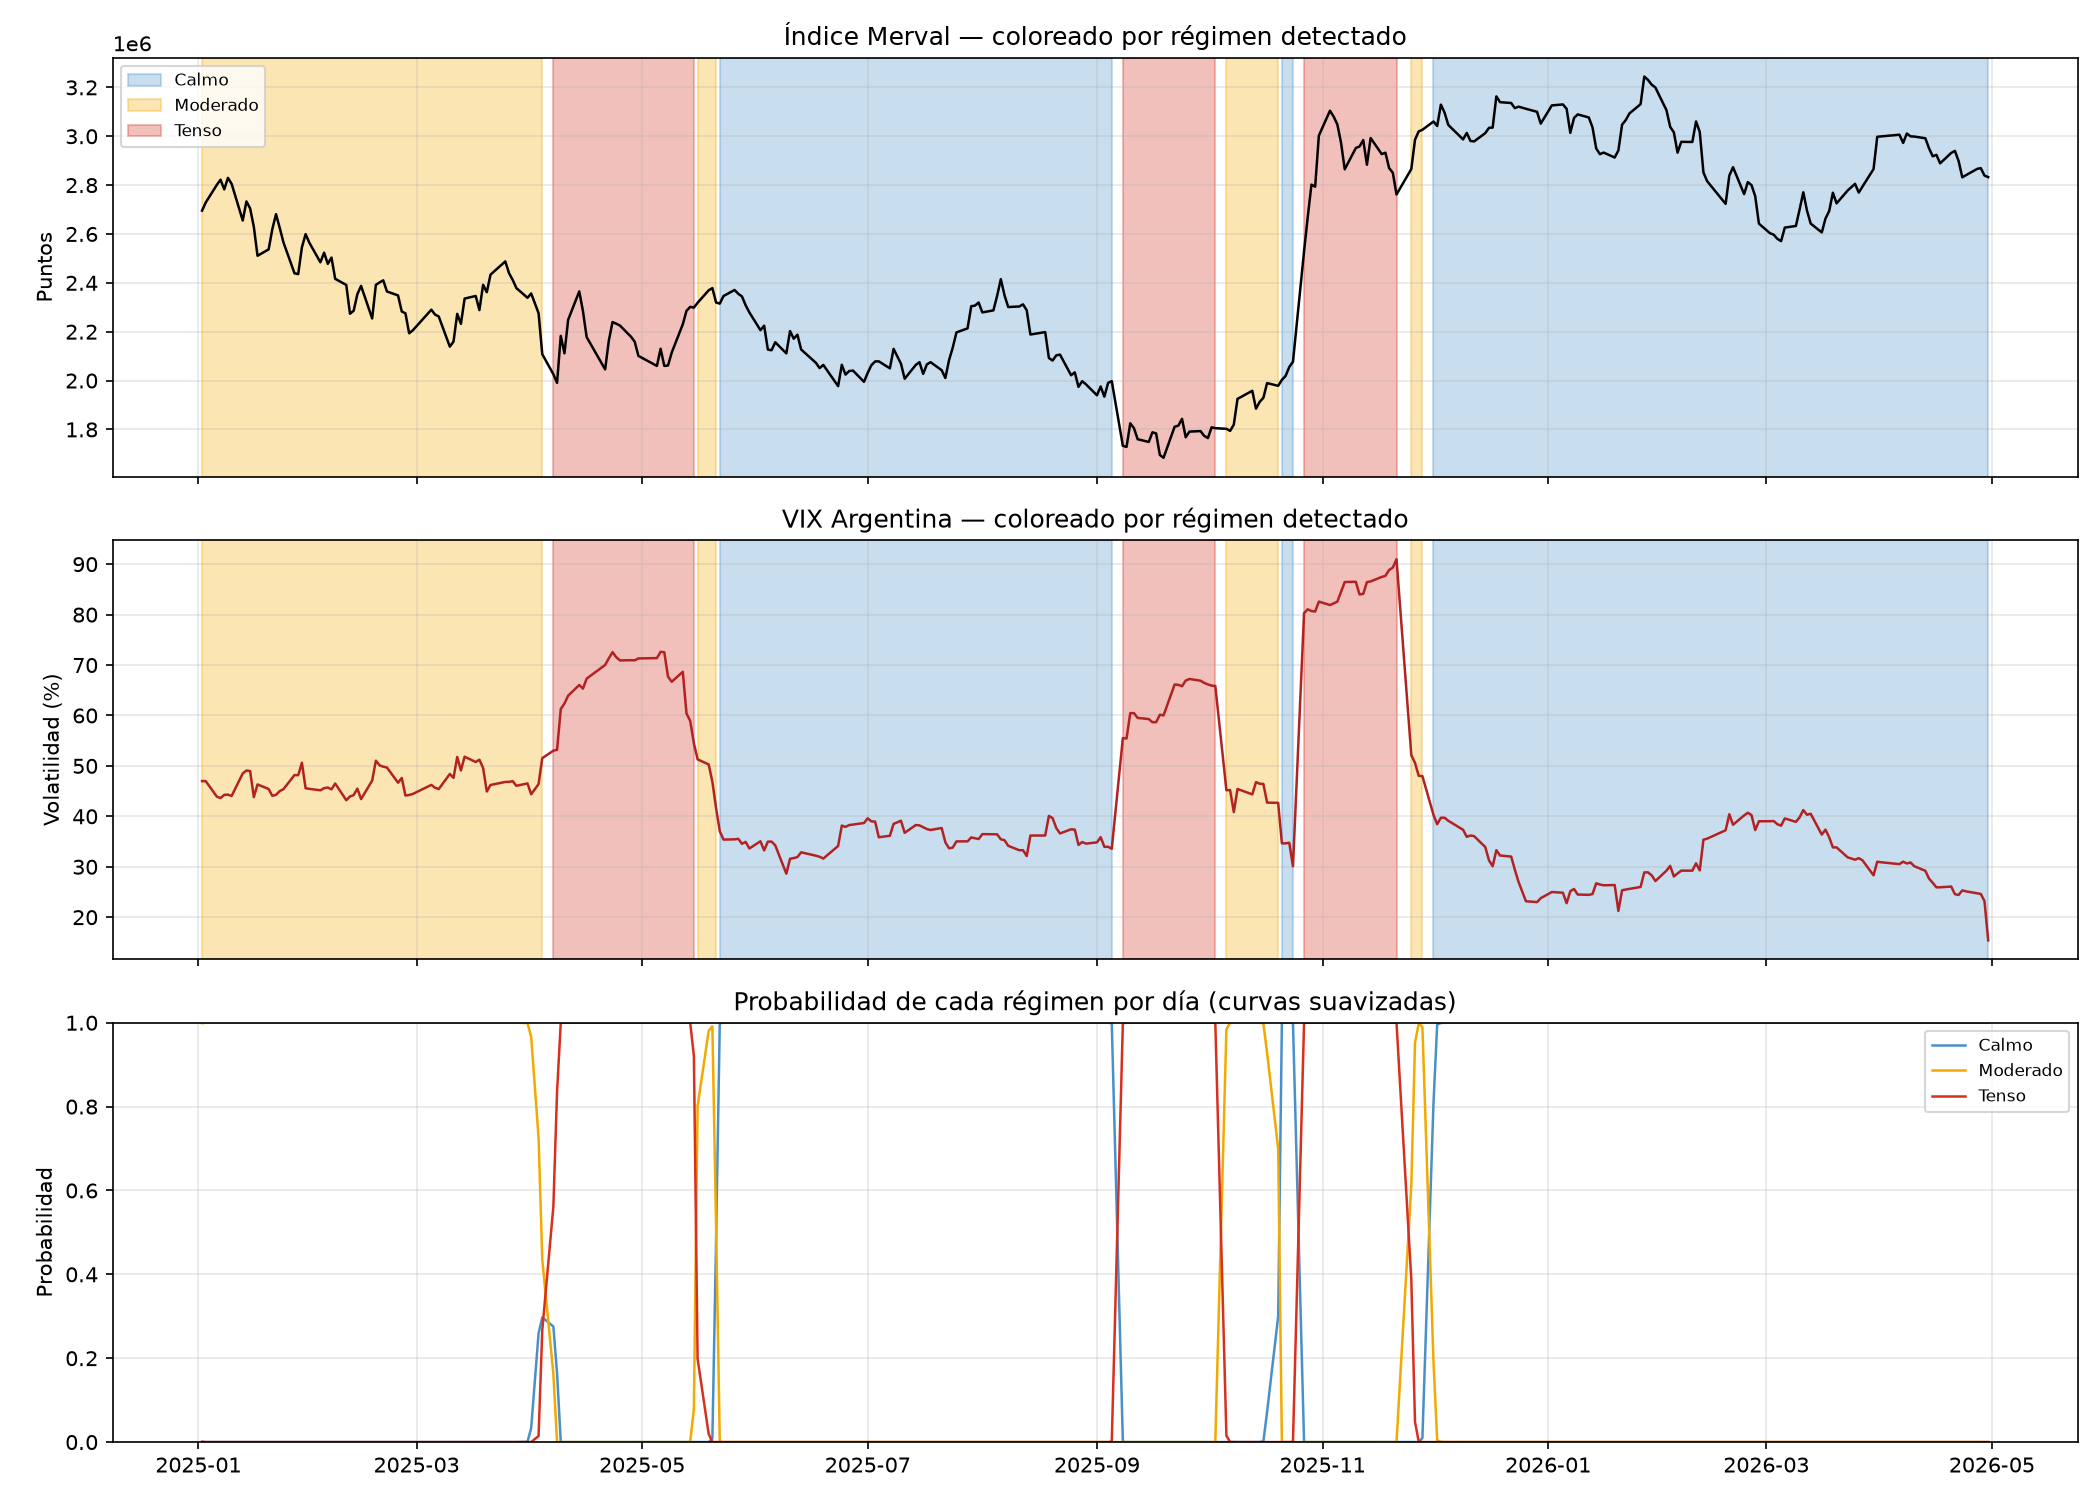
\includegraphics[width=0.9\linewidth]{hmm_regimen_mercado.png}
\caption{S\&P~Merval y VIX argentino coloreados por régimen, y probabilidad suavizada de cada
régimen por día. Fuente: elaboración propia (\carpeta{Lado Bursatil/06_hmm_regimen_mercado}).}
\label{fig:hmm}
\end{figure}

\subsubsection{Estacionariedad}

Con tres años de datos, 46 de los 47 precios no son estacionarios (ADF con constante y
tendencia) y los 47 retornos sí lo son (ADF con constante; 43 con $p<0{,}0001$ y el más alto
con $p=0{,}006$). La única excepción en precios, TGSU2 ($p=0{,}047$), está dentro de lo que se
espera por azar en 47 pruebas. Los modelos usan, entonces, retornos y no precios
\citep{zablotsky2002,worthington2003}.

En la ventana de la unión se repitió la prueba con ADF y KPSS sobre 156 series
(tabla~\ref{tab:u5}). Retornos, volumen anormal y tono de cada empresa son estables. El tono de
las noticias en nivel dio \textit{inconcluso} ($p=0{,}35$ en el ADF, sin problemas en el KPSS)
porque cambia en ciclos de meses: el promedio trimestral fue de $+7{,}5$ en el segundo
trimestre de 2025, $+0{,}5$ en el tercero, $+7{,}6$ en el cuarto, $+3{,}7$ en el primero de
2026 y $-2{,}9$ en abril de 2026. Con un año de datos, la prueba no distingue un clima que va
y viene de uno que se va corriendo, un rasgo conocido de las series de tono
\citep{correarocha2026}. Por eso el VAR usa el \textit{tono anormal}, que es estable sin
discusión ($p<0{,}0001$) y mide la sorpresa —lo que puede mover precios— en lugar del clima de
fondo; el tono en nivel quedó como prueba de robustez. El VIX también dio inconcluso, por la
misma razón, y entra a los modelos solo a través del régimen.

\begin{table}[H]
\centering\small
\begin{tabular}{@{}lrlll@{}}
\toprule
\textbf{Serie} & \textbf{Datos} & \textbf{ADF (p)} & \textbf{KPSS (p)} & \textbf{Conclusión} \\
\midrule
Retorno del S\&P~Merval & 244 & $<$0,0001 & $\geq$0,10 & Estacionaria \\
Monto operado anormal & 244 & $<$0,0001 & $\geq$0,10 & Estacionaria \\
Atención anormal & 224 & 0,0014 & 0,077 & Estacionaria \\
Notas por rueda & 244 & 0,0044 & $\leq$0,01 & Estacionaria con memoria \\
Tono anormal (variable del VAR) & 224 & $<$0,0001 & $\geq$0,10 & Estacionaria \\
Tono en nivel & 244 & 0,3492 & $\geq$0,10 & Inconclusa \\
Cambio de tono & 243 & $<$0,0001 & $\geq$0,10 & Estacionaria \\
VIX argentino & 244 & 0,1545 & 0,095 & Inconclusa \\
\midrule
Retorno (47 acciones) & 47 series & \multicolumn{3}{l}{47 estacionarias} \\
Volumen anormal (47 acciones) & 47 series & \multicolumn{3}{l}{46 estacionarias y 1 con memoria} \\
Tono propio (17 empresas) & 17 series & \multicolumn{3}{l}{14 estacionarias y 3 con memoria} \\
\bottomrule
\end{tabular}
\caption{Estacionariedad de las series en la ventana de la unión. Fuente: elaboración propia
(\carpeta{Unión/05_adf_union}).}
\label{tab:u5}
\end{table}

\subsubsection{Relaciones entre tono, retorno y volumen}

Dos correlaciones adelantan los resultados. En el VAR del mercado, las sorpresas del tono y
del retorno de una misma rueda están correlacionadas (0,19): se mueven juntas dentro de la
rueda. Y el tono de las notas publicadas de noche, con el mercado cerrado, tiene una
correlación de 0,42 con el retorno de ese mismo día: después de una rueda buena, las notas de
la noche son más positivas. Con datos diarios, la primera correlación no dice quién movió a
quién; la segunda ya sugiere que las notas de la noche cuentan cómo cerró el mercado. La
figura~\ref{fig:u4} muestra las series juntas.

\begin{figure}[H]
\centering
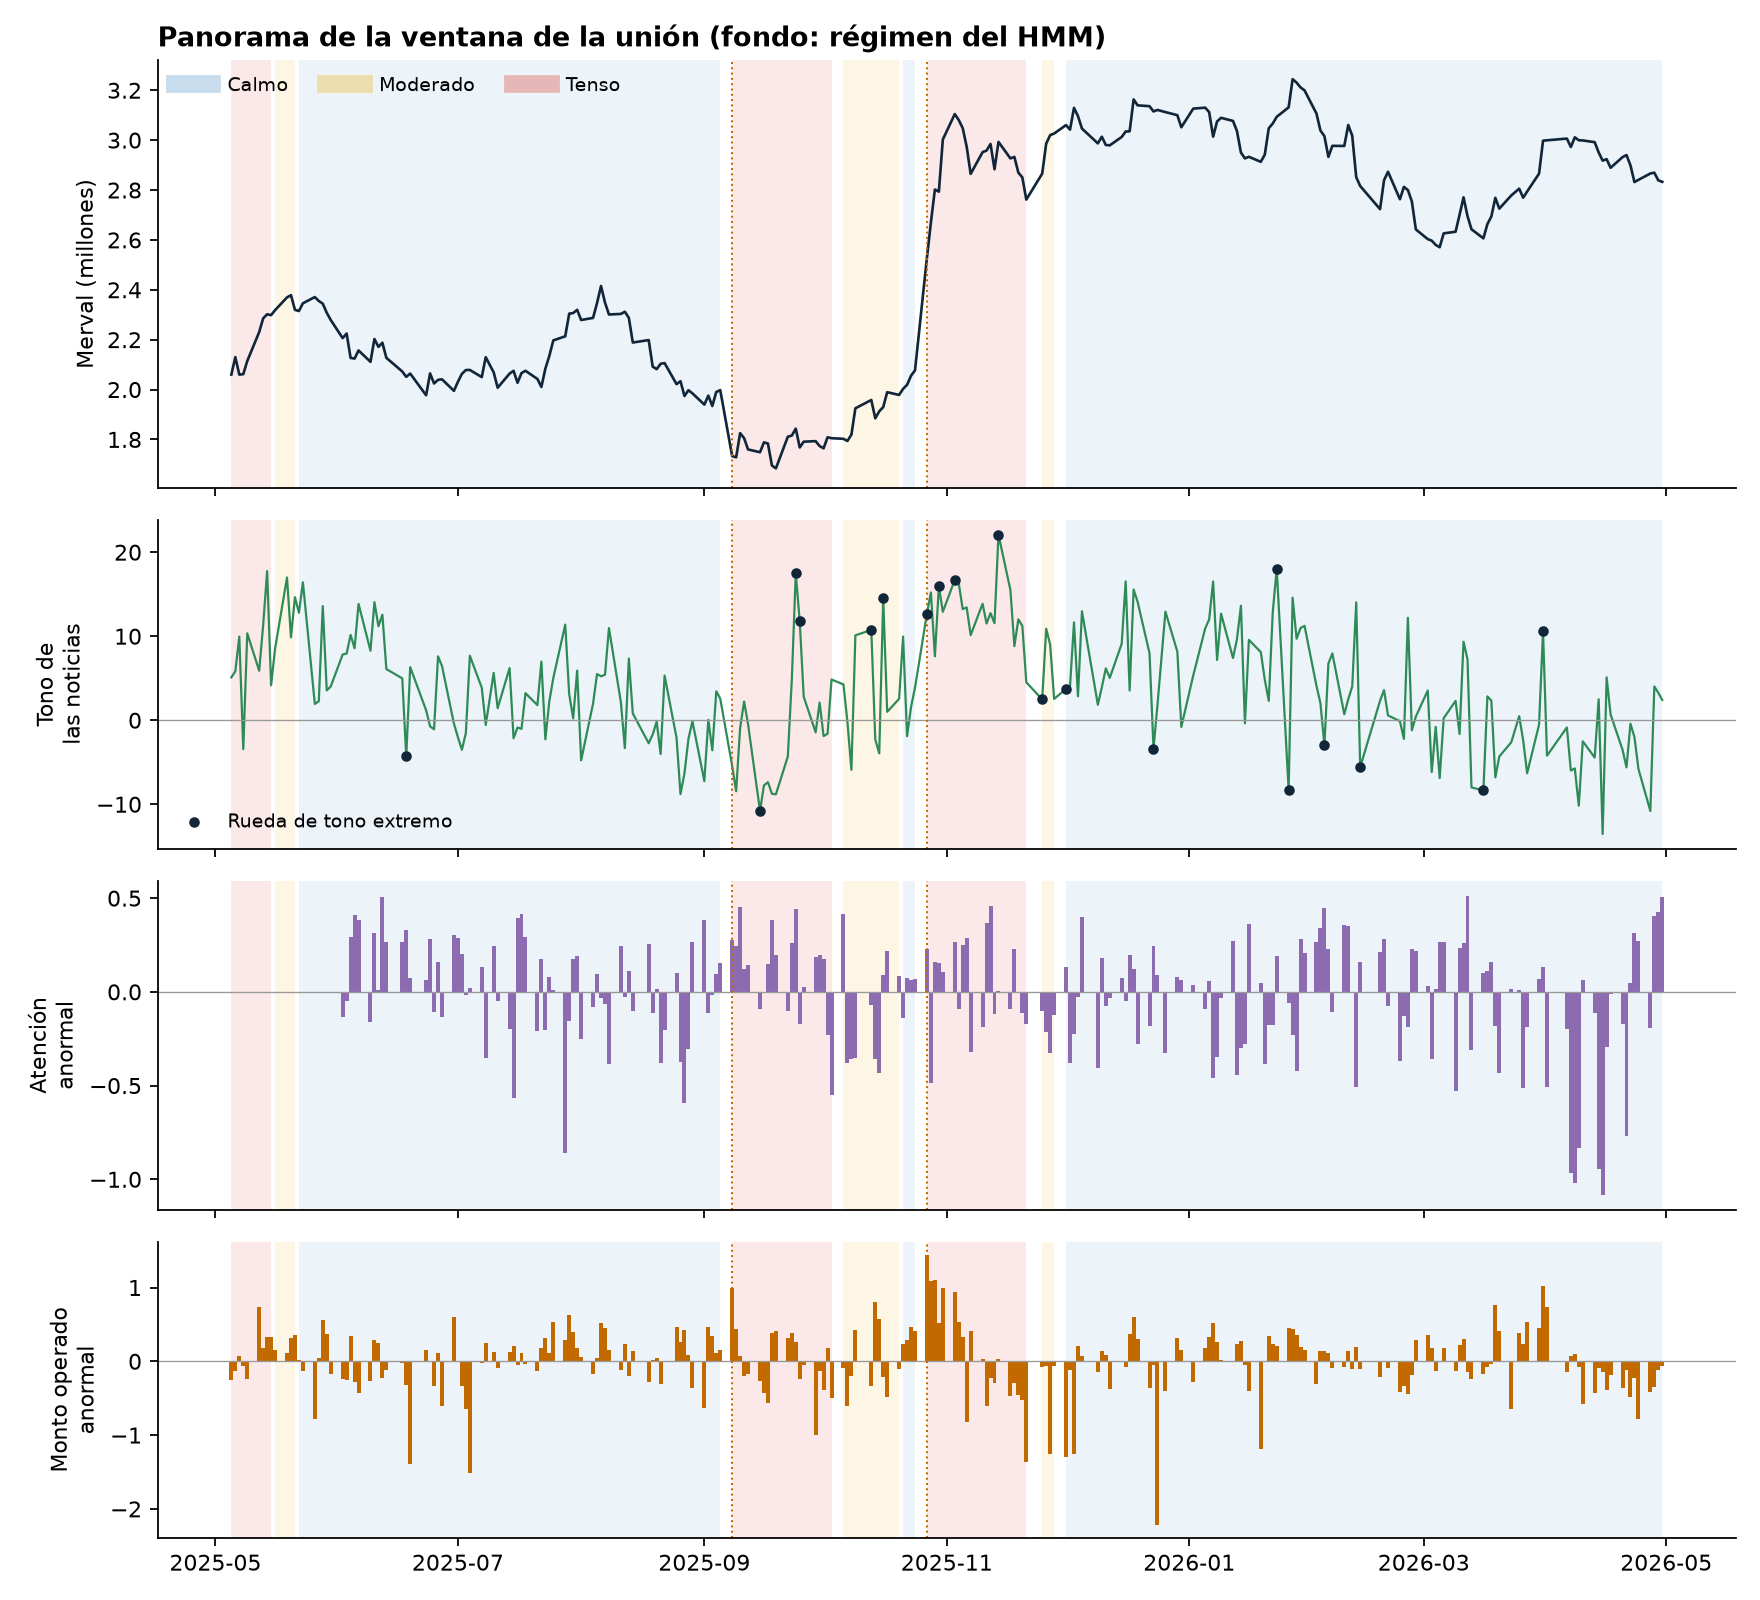
\includegraphics[width=0.88\linewidth]{u4_panorama.png}
\caption{S\&P~Merval, tono de las noticias, atención de los medios y monto operado anormal en
la ventana de la unión. El color de fondo es el régimen; las líneas punteadas, los días
electorales. Fuente: elaboración propia (\carpeta{Unión/04_dataset_unificado}).}
\label{fig:u4}
\end{figure}

% ---------------------------------------------------------------------
\subsection{Modelado}
\label{sec:modelado}

\subsubsection{FinBETO: etiquetado, entrenamiento y evaluación}
\label{sec:finbeto-modelo}

\textbf{Clases.} Se trabajó con cuatro clases: positiva (POS), negativa (NEG), neutra (NEU) y
mixta (MIXTO). Una parte de las oraciones de la prensa económica combina señales de ambos
signos —por ejemplo, un dato de actividad que mejora mientras la inflación se acelera— y
forzarlas a una sola clase habría sido arbitrario.

\textbf{Etiquetado.} Se etiquetó con Gemma (\texttt{gemma4:26b}, temperatura 0,1) en dos
pasos por noticia. Primero, el modelo leyó el título, la bajada y los primeros 3.000
caracteres, y produjo un análisis de contexto (tema central, encuadre, actores y tono general).
Después etiquetó cada oración de al menos 30 caracteres, con ese contexto como referencia y la
instrucción de que el sentimiento surgiera de lo que la oración expresa por sí misma. El
criterio es, por lo tanto, relativo al encuadre de cada nota. Se tomó un artículo de cada una
de las nueve fuentes por lote, hasta 408 noticias (45 o 46 por fuente) y 11.605 filas
etiquetadas: 46,4\% NEU, 23,8\% POS, 20,8\% NEG y 8,9\% MIXTO.

\textbf{Entrenamiento.} Para que la clase neutra no dominara, se tomó una muestra balanceada
de hasta 2.400 oraciones por clase (todas las de MIXTO), dividida en 80\% para entrenamiento,
10\% para validación y 10\% para prueba (6.588, 824 y 824 oraciones). La pérdida se ponderó por
la raíz cuadrada de la frecuencia inversa de cada clase. El preentrenamiento continuado se
hizo con la tarea MLM (15\% de los tokens enmascarados) sobre el texto de los 14.667 artículos
del corpus antes de su depuración final: 3 épocas, segmentos de 128 tokens y tasa de
aprendizaje $2\cdot10^{-5}$. La pérdida de evaluación bajó de 1,233 a 1,121, y ante la frase
«La [MASK] llegó al 3\% mensual según el INDEC» el modelo propuso «inflación» con probabilidad
0,81. El ajuste fino usó 5 épocas, lotes de 32, tasa de aprendizaje $2\cdot10^{-5}$ con 10\%
de calentamiento, decaimiento de pesos 0,01 y selección de la mejor época por F1 macro en
validación.

\textbf{Problemas de la evaluación original.} La primera evaluación informó un F1 macro de
0,7296 en cuatro clases, frente a 0,6201 del modelo de referencia. Al revisarla se encontraron
tres problemas: la división se había hecho por oración y no por noticia (las 824 oraciones de
prueba venían de 337 noticias que también aportaban oraciones al entrenamiento); había textos
repetidos (41 oraciones de prueba, el 5\%, estaban también en entrenamiento); y había restos
del \textit{scraping} etiquetados como neutros («PUBLICIDAD PUBLICIDAD PUBLICIDAD», «Sobre la
firma Newsletter Clarín»). Es el problema de fuga de información descrito por
\citet{kapoor2023leakage}.

\textbf{Nueva medición.} Sin modificar el modelo en uso, se limpió el conjunto etiquetado (se
descartaron 750 filas de relleno o repetidas y quedaron 10.855 oraciones), se lo dividió
\textit{por noticia} (330 noticias para entrenamiento, 39 para validación y 39 para prueba,
sin textos compartidos) y se reentrenó solo para medir, con tres semillas por división. El
código reproduce el resultado original (0,732 con la división por oración). Con la división por
noticia, el F1 macro es de 0,685 (tabla~\ref{tab:finbeto}). Para comparar en igualdad de
condiciones con el modelo de referencia, que tiene tres clases, se usaron solo las oraciones
POS, NEG y NEU, contando como error cada predicción MIXTO de FinBETO: sobre noticias no vistas,
FinBETO obtiene 0,724 y el de referencia 0,546. El de referencia, entrenado con tuits, clasifica
como neutras 411 de las 662 oraciones.

\begin{table}[H]
\centering\footnotesize
\begin{tabular}{@{}lcc@{}}
\toprule
\textbf{Medida (prueba, media de 3 semillas)} & \textbf{División por oración} & \textbf{División por noticia} \\
\midrule
F1 macro, 4 clases & 0,732 $\pm$ 0,012 & \textbf{0,685 $\pm$ 0,009} \\
Exactitud & 0,743 & 0,691 \\
F1 POS / NEG / NEU / MIXTO & 0,752 / 0,760 / 0,754 / 0,663 & 0,694 / 0,677 / 0,725 / 0,645 \\
\midrule
F1 macro, 3 clases: FinBETO & 0,773 & \textbf{0,724} \\
F1 macro, 3 clases: modelo de referencia & 0,620 & 0,546 \\
\bottomrule
\end{tabular}
\caption{Calidad de FinBETO según cómo se dividen los datos. La estimación que corresponde
informar es la de la división por noticia. Fuente: elaboración propia a partir de
\carpeta{Lado Noticias/sentimiento_finbert}.}
\label{tab:finbeto}
\end{table}

\textbf{Aplicación al corpus.} El modelo se aplicó a todas las oraciones del corpus de entre 30
y 600 caracteres, incluido el título. Se excluyeron 2.438 oraciones de relleno (firmas de
Clarín, marcas de publicidad de Infobae) y quedaron 399.803. Para cada artículo se calculó el
sentimiento neto: el porcentaje de oraciones positivas menos el de negativas; las mixtas y las
neutras no suman ni restan. La serie diaria original promedia ese valor por fecha: abarca 487
días, 377 con datos, y marca 36 shocks (17 positivos y 19 negativos) con una banda de 1,5
desvíos sobre los siete días previos. La unión no usa esa serie sino la clasificación por
oración, reagrupada por rueda.

\subsubsection{Reconocimiento de entidades y cruce con el sentimiento}
\label{sec:ner-modelo}

El NER combinó el modelo estadístico de spaCy con dos \textit{gazetteers}: uno de 160
indicadores económicos en seis categorías (macroeconomía, política monetaria, política
fiscal, mercado financiero, mercado laboral y precios y pobreza) y uno de las 47 empresas del
panel, \textit{canonicalizado}: cada alias (razón social, nombre comercial, ticker) se resuelve
al ticker, para que «Banco Galicia», «Grupo Financiero Galicia» y «GGAL» cuenten como una sola
entidad. Para limitar los falsos positivos, los alias en mayúsculas se buscan respetando
mayúsculas (sin esta regla, el alias AGRO coincidía con la palabra «agro» en 920 artículos), se
excluyeron alias que son palabras comunes («Hipotecario», «Molinos») y las entidades del modelo
que coinciden con un término del \textit{gazetteer} no se cuentan dos veces.

La limpieza del NER resolvió tres tipos de ruido (tabla~\ref{tab:ner}): el texto de relleno del
\textit{scraping} («PUBLICIDAD» era la organización más mencionada del corpus), las
autorreferencias de cada medio y los fragmentos sin valor informativo que detecta el modelo
estadístico. Para el modelo estadístico se exigió una forma válida (no solo números ni más de
seis palabras), al menos dos artículos con la entidad y un único tipo por cadena.

\begin{table}[H]
\centering\footnotesize
\begin{tabular}{@{}lll@{}}
\toprule
 & \textbf{Antes del filtrado} & \textbf{Después} \\
\midrule
Entidades únicas & 65.352 & 17.894 \\
Menciones de «PUBLICIDAD» como entidad & 2.258 (primera del ranking) & 0 \\
«newsletter clarín» como entidad & 2.134 artículos & 0 \\
Empresas del panel & 20, fragmentadas en variantes & 47, canonicalizadas por ticker \\
Tickers con menciones en el corpus & — & 44 de 47 \\
Falsos positivos del alias AGRO & 920 artículos & 0 \\
\bottomrule
\end{tabular}
\caption{Efecto de la limpieza del reconocimiento de entidades. Fuente: elaboración propia a
partir de \carpeta{Lado Noticias/ner_entidades}.}
\label{tab:ner}
\end{table}

Cada mención se unió con el sentimiento de la oración que la contiene, por artículo y número
de oración y exigiendo que el texto coincida: se cruzaron 243.265 de las 244.809 oraciones con
entidades (99,37\%). Antes de agregar, 24 variantes de indicadores se unificaron en su forma
más frecuente (por ejemplo, «PIB» y «producto bruto interno» en «PBI»; «CCL» y «contado con
liquidación»). Entre las empresas más mencionadas, el sentimiento neto fue de $+28{,}9$ para
Galicia, $+25{,}0$ para Macro y $+17{,}4$ para YPF, y cercano a cero para Supervielle
($+1{,}4$) y Edenor ($+0{,}9$). Debe leerse como el tono del contexto en que aparece la
entidad y no como una opinión sobre ella.

\subsubsection{VAR, Granger e impulso-respuesta}

Se usaron las 224 ruedas del 02/06/2025 al 30/04/2026: las 244 de la unión menos las primeras
20, que no tienen tono anormal ni atención. Se estimaron VAR en cinco niveles
(tabla~\ref{tab:niveles-var}), siempre en las dos direcciones y para precio y volumen. En
total se hicieron 304 pruebas de Granger, corregidas por Benjamini-Hochberg dentro de cada
nivel.

\begin{table}[H]
\centering\small
\begin{tabularx}{\linewidth}{@{}L{2.4cm}YC{1.8cm}@{}}
\toprule
\textbf{Nivel} & \textbf{Variables del VAR} & \textbf{Modelos} \\
\midrule
Mercado & Tono anormal, atención anormal, retorno del S\&P~Merval y monto operado anormal & 1 \\
Empresa & Tono anormal del mercado, retorno y volumen anormal de la acción & 47 \\
Tono propio & Lo anterior más el tono propio de la empresa & 17 \\
Sector & Tono anormal, retorno y volumen anormal promedio del sector & 10 \\
Régimen & Todas las ruedas, con una marca de día Tenso que interactúa con los rezagos & 4 regresiones \\
\bottomrule
\end{tabularx}
\caption{Niveles del análisis VAR. Fuente: elaboración propia (\carpeta{Unión/06_var_granger}).}
\label{tab:niveles-var}
\end{table}

Para el régimen no se separaron los días de cada uno, porque eso pegaría días no
consecutivos. Se usaron todos los días con una marca de día Tenso y se probó el efecto en los
días Calmo, en los Tenso y la diferencia. Como control de calibración, el test por empresa se
repitió con el tono mezclado al azar (1.880 pruebas): debería dar $p<0{,}05$ en alrededor del
5\% de los casos si el test no inventa resultados. Todos los VAR resultaron estables (raíces
dentro del círculo unitario).

\subsubsection{Notas publicadas con el mercado cerrado}

Dentro de una misma rueda el tono y el retorno se mueven juntos, y con datos diarios no se
sabe quién movió a quién. Para resolverlo se usó la hora de cada nota. Las notas publicadas
entre el cierre de la rueda anterior y la apertura salen antes de cualquier operación de la
rueda: el precio de esa rueda no puede haberlas causado. Si su tono anticipa el salto de
apertura, eso es noticias \flecha{} mercado sin ambigüedad, en la línea de
\citet{glasserman2025}. La especificación se escribió y guardó antes de correr ningún cálculo
(anexo~\ref{anx:especificaciones}):

\begin{itemize}
  \item \textbf{Notas:} las asignadas a la rueda que no se publicaron durante la sesión
        (11:00 a 17:00), sin las de hora sospechosa: 8.069 notas; todas las ruedas tienen
        alguna (mediana 29).
  \item \textbf{Variables:} el tono anormal de esas notas y, para las 17 empresas, su tono
        propio con solo esas notas; el retorno de apertura (del cierre de ayer a la apertura de
        hoy) y el de la sesión (de la apertura al cierre). El mercado es el promedio de las 47
        acciones, porque los datos no traen la apertura del índice.
  \item \textbf{Modelo:} mínimos cuadrados con errores robustos; controla por el retorno del
        día anterior, porque muchas notas de la noche cuentan cómo cerró el mercado, y por si
        la rueda viene de un día sin mercado. En el panel de empresas, con efecto fijo por
        empresa y errores agrupados por rueda.
  \item \textbf{Evidencia a favor de la hipótesis:} que el tono anticipe el retorno de
        apertura con signo positivo y $p<0{,}05$ tras la corrección. Se informa también el
        resultado sin los dos días electorales.
\end{itemize}

\subsubsection{Estudios de eventos}

\textbf{Ruedas de tono extremo (U7).} Se usaron dos tipos de eventos. Para el mercado, las
ruedas de tono extremo de la sección~\ref{sec:tono-rueda} (18 eventos, contando como uno las
ruedas seguidas del mismo signo), medidas sobre el propio S\&P~Merval con el modelo de media
constante: un modelo de mercado restaría justamente el movimiento del índice y el efecto
buscado desaparecería por construcción. Para las 17 empresas, las ruedas en que se habló de
ellas mucho mejor o peor que del mercado (más de 2,5 desvíos de su propio tono propio): 88
eventos, medidos con el modelo de mercado de cada acción. La ventana $[-3,+5]$ se partió en
antes $[-3,-1]$, día $[0]$ y después $[+1,+5]$.

Una primera corrida mostró una suba de 6,3\% en las ruedas previas a los eventos positivos,
generada casi entera por un solo evento cuya ventana incluía el salto de 21\% posterior a las
legislativas. Un salto así, además, infla el «promedio normal» de los eventos siguientes. Por
eso los dos días electorales se excluyeron de las ventanas de estimación y los eventos cuya
ventana incluye uno se analizaron aparte. Quedaron 16 eventos de mercado: 7 positivos y 9
negativos.

\textbf{Shock de cantidad de noticias (U7b).} Es la prueba con la definición literal del
plan: el puntaje $z$ de la cantidad de notas de la rueda contra las 30 ruedas previas, con
umbral $z>2$; para cada empresa, la cantidad de artículos que la mencionan, con al menos 3 en
la rueda. Un shock de cantidad no tiene signo —muchas notas pueden ser buenas o malas—, así que
la medida central es el tamaño del movimiento del precio el día del shock, en valor absoluto,
además del volumen. La significancia se evalúa contra fechas al azar y con Benjamini-Hochberg
sobre las 14 pruebas principales. La especificación se escribió antes de calcular los
resultados.

La versión original mostró un problema: los 13 eventos de mercado caían todos en la primera
rueda después de un día sin mercado. Por la regla de las 17:00, esa rueda junta las notas de
tres o cuatro días, de modo que casi siempre «tiene muchas más notas». La regla marcaba fines
de semana, no noticias. Se corrigió midiendo la cantidad \textit{por día de calendario} (la
cantidad de la rueda dividida por los días que cubre), lo más fiel al «volumen diario» del
plan. El cambio quedó registrado con su fecha y su motivo, y la versión original se informa
también. Se agregó, antes de correrla, una prueba que cuenta solo las notas publicadas con el
mercado cerrado y mide el salto de apertura, el único precio que se forma después de esas notas
y antes de las de la sesión.

\subsubsection{Robustez}

La prueba de robustez (U8) cambia una sola decisión por vez y mira si la conclusión sigue en
pie: tono ajustado por portal, tono en nivel, sin notas de hora sospechosa, fecha de calendario
en lugar de la regla de las 17:00, solo notas del día antes del cierre, sin abril de 2026,
días electorales como control, sin las cuatro acciones ilíquidas, régimen filtrado, Calmo
contra No calmo y umbrales 2 y 3 para las ruedas de tono extremo. Antes de cambiar nada, el
script rearma todo con las decisiones originales y comprueba que reproduce los resultados
principales, de modo que las diferencias se deben a la decisión cambiada y no al código.
